\section{System Architecture}

Our investigation into a robust zero-shot HMLC framework followed an iterative design process. We began by analyzing a promising top-down prompting approach, then developed a traceable self-refining pipeline, and finally, upon identifying its limitations, engineered a more robust multi-agent ensemble.

\subsection{Baseline Inspiration: Top-Down Zero-Shot Classification}

A promising recent approach to HMLC, which we refer to as H3Prompting, was introduced by \citet{singh-etal-2025-gatenlp}. This method decomposes the hierarchical classification task into a sequence of zero-shot LLM queries, where an initial prompt determines the top-level category, and subsequent prompts classify second-level narratives conditioned on the first-level prediction. In the spirit of reproducible research, we first aimed to replicate this method. However, the lack of publicly available implementation details prevented a direct reproduction, motivating our development of an open and configurable framework to systematically investigate zero-shot HMLC strategies.

\subsection{Initial Approach: The Traceable Actor-Critic Pipeline}

Our first architectural exploration, the Actor-Critic Pipeline, sought to improve the reliability and transparency of a single agent's output. While zero-shot classification is powerful, simple label outputs lack traceability, making them difficult to audit and susceptible to unverified hallucinations. To overcome this, we designed a multi-stage pipeline that reframes the task from simple classification to evidence-grounded claim generation and validation.

Our implementation uses the LangGraph framework to structure the process as a cyclical state graph \citep{langgraph2024}. The pipeline configuration is managed by a \texttt{ConfigurableGraphBuilder}, allowing components like validation to be enabled or disabled and different LLMs to be assigned to specific nodes via a YAML file. The workflow proceeds through several stages, as illustrated in Figure~\ref{fig:actor_critic_pipeline}.

\begin{figure}[!ht]
\centering
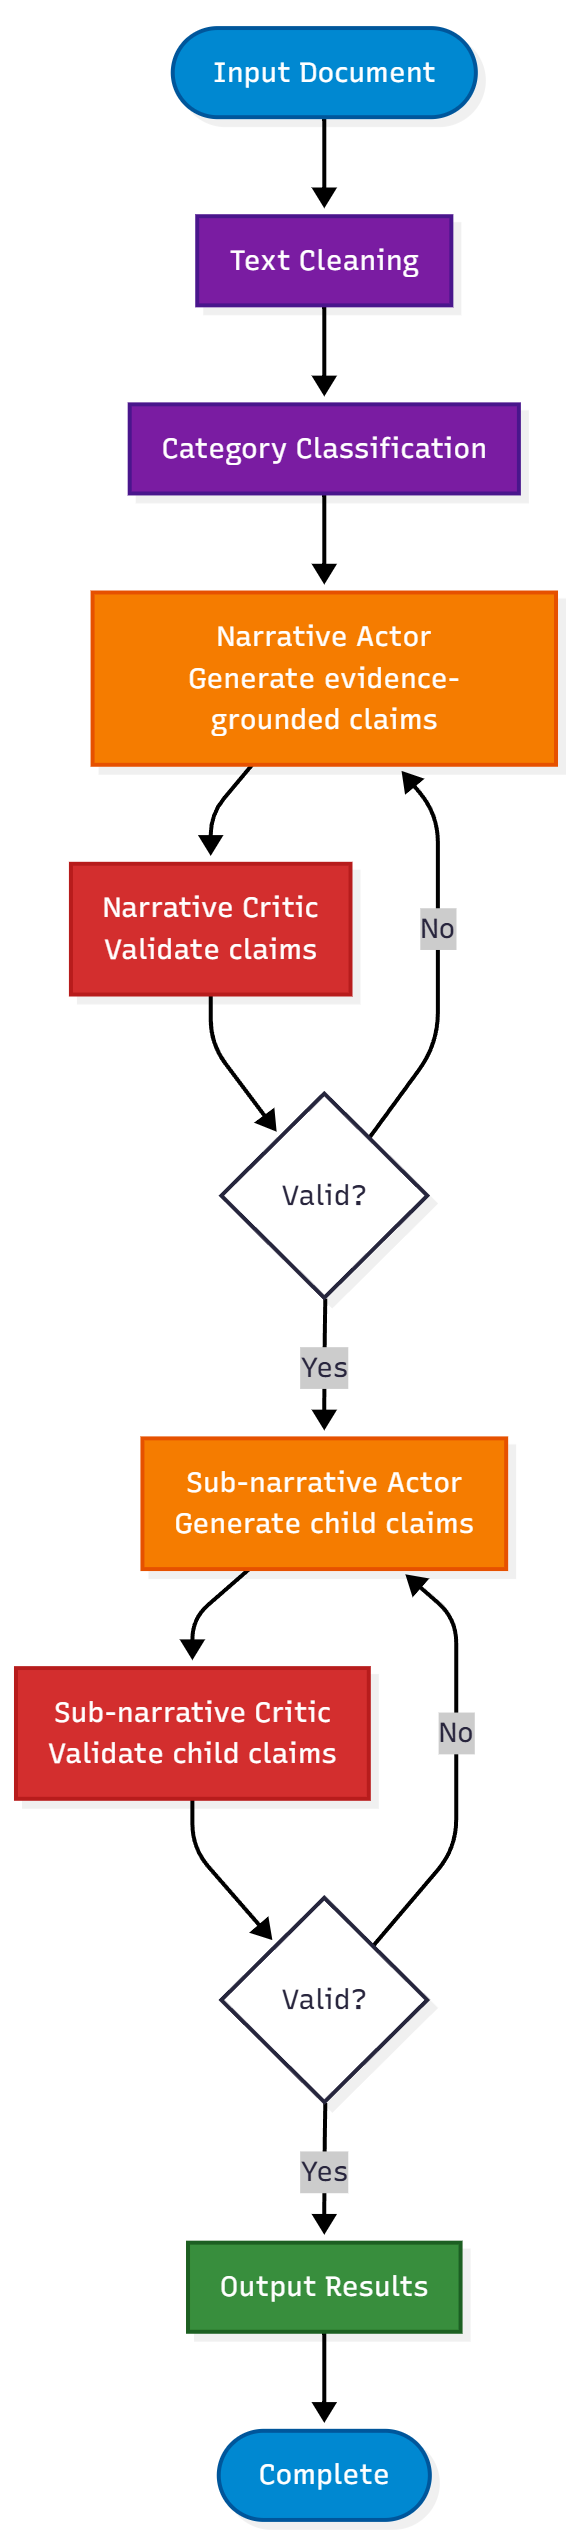
\includegraphics[height=20cm]{assets/diagrams/actor-critique.png}
\caption{Actor-Critic validation pipeline architecture. The system decomposes HMLC into hierarchical stages where a Narrative Actor generates evidence-grounded claims, which are then validated by a Narrative Critic. Feedback loops enable iterative refinement before progressing to sub-narrative classification.}
\label{fig:actor_critic_pipeline}
\end{figure}

\subsubsection{Category Classification}

An initial node determines the document's high-level topic (e.g., CC or URW) to focus subsequent stages on the relevant subset of the narrative taxonomy.

\subsubsection{The Narrative Actor (Claim Generation)}

The ``Actor'' is an LLM agent prompted to act as an expert analyst. For each narrative it identifies, it must generate a structured JSON object containing the \texttt{narrative\_name}, a verbatim \texttt{evidence\_quote} from the text, and reasoning that connects the two.

\subsubsection{The Narrative Critic (Claim Validation)}

The Actor's output is passed to the ``Critic,'' a separate LLM agent with a distinct, skeptical persona. The Critic validates the Actor's claims against strict criteria (evidence accuracy, relevance, completeness). If the Critic finds flaws, it generates structured feedback, and the graph's conditional logic routes the state back to the Actor for a retry, incorporating the feedback into a refinement prompt.

\subsubsection{Sub-narrative Actor and Critic}

Once narratives are approved, the process repeats hierarchically. A Sub-narrative Actor generates claims for each parent narrative, which are then validated by a Sub-narrative Critic, also with a self-correction loop.

This evidence-grounded architecture offers significant advantages in traceability and auditability, as every prediction is grounded in a textual \texttt{evidence\_quote}, a process we enhanced using LangSmith for detailed debugging and prompt refinement \citep{langsmith2024}. However, while this pipeline showed promise, our experiments revealed that it introduced its own form of instability. The process was highly sensitive to the quality of the Critic's feedback, which, being LLM-generated, was itself prone to stochasticity. A flawed critique could send the Actor down an unproductive refinement path, sometimes degrading performance. This reliance on a single, fallible ``critic'' highlighted a fundamental bottleneck and motivated our shift towards a more robust consensus mechanism.

\subsection{Proposed Framework: The Agora Multi-Agent Ensemble}

To overcome the limitations of a single-critic system and the broader issue of single-agent stochasticity, we developed Agora, a multi-agent ensemble framework. The core principle of Agora is to replace the judgment of a single agent (or a single critic) with the collective ``wisdom of the crowd,'' leveraging the consensus of multiple independent agents to arrive at a more stable and accurate classification.

The framework operates via a fan-out, fan-in process for each level of the hierarchy (e.g., Narrative classification).

\subsubsection{Fan-Out (Parallel Classification)}

Instead of a single LLM call, Agora instantiates $N$ independent agents (where $N$ is a configurable parameter). The same input text and prompt are sent to all $N$ agents, who perform the classification in parallel. This step effectively samples $N$ independent points from the LLM's output distribution for the given task.

\subsubsection{Fan-In (Aggregation via Voting)}

After all $N$ agents return their individual classifications, an Aggregation node consolidates the results using a voting scheme. We implemented and evaluated three distinct aggregation strategies:

\begin{itemize}
\item \textbf{Union:} The final label set includes any label proposed by at least one agent. This high-recall strategy is useful for identifying all potential labels.

\item \textbf{Intersection:} The final label set includes only those labels that all agents unanimously agreed upon. This high-precision strategy filters out all but the most confident predictions.

\item \textbf{Majority Vote:} The final label set includes any label proposed by more than half ($> N/2$) of the agents. This strategy provides a robust balance between precision and recall, filtering out stochastic, outlier classifications while retaining a strong consensus.
\end{itemize}

\begin{figure*}[!ht]
\centering
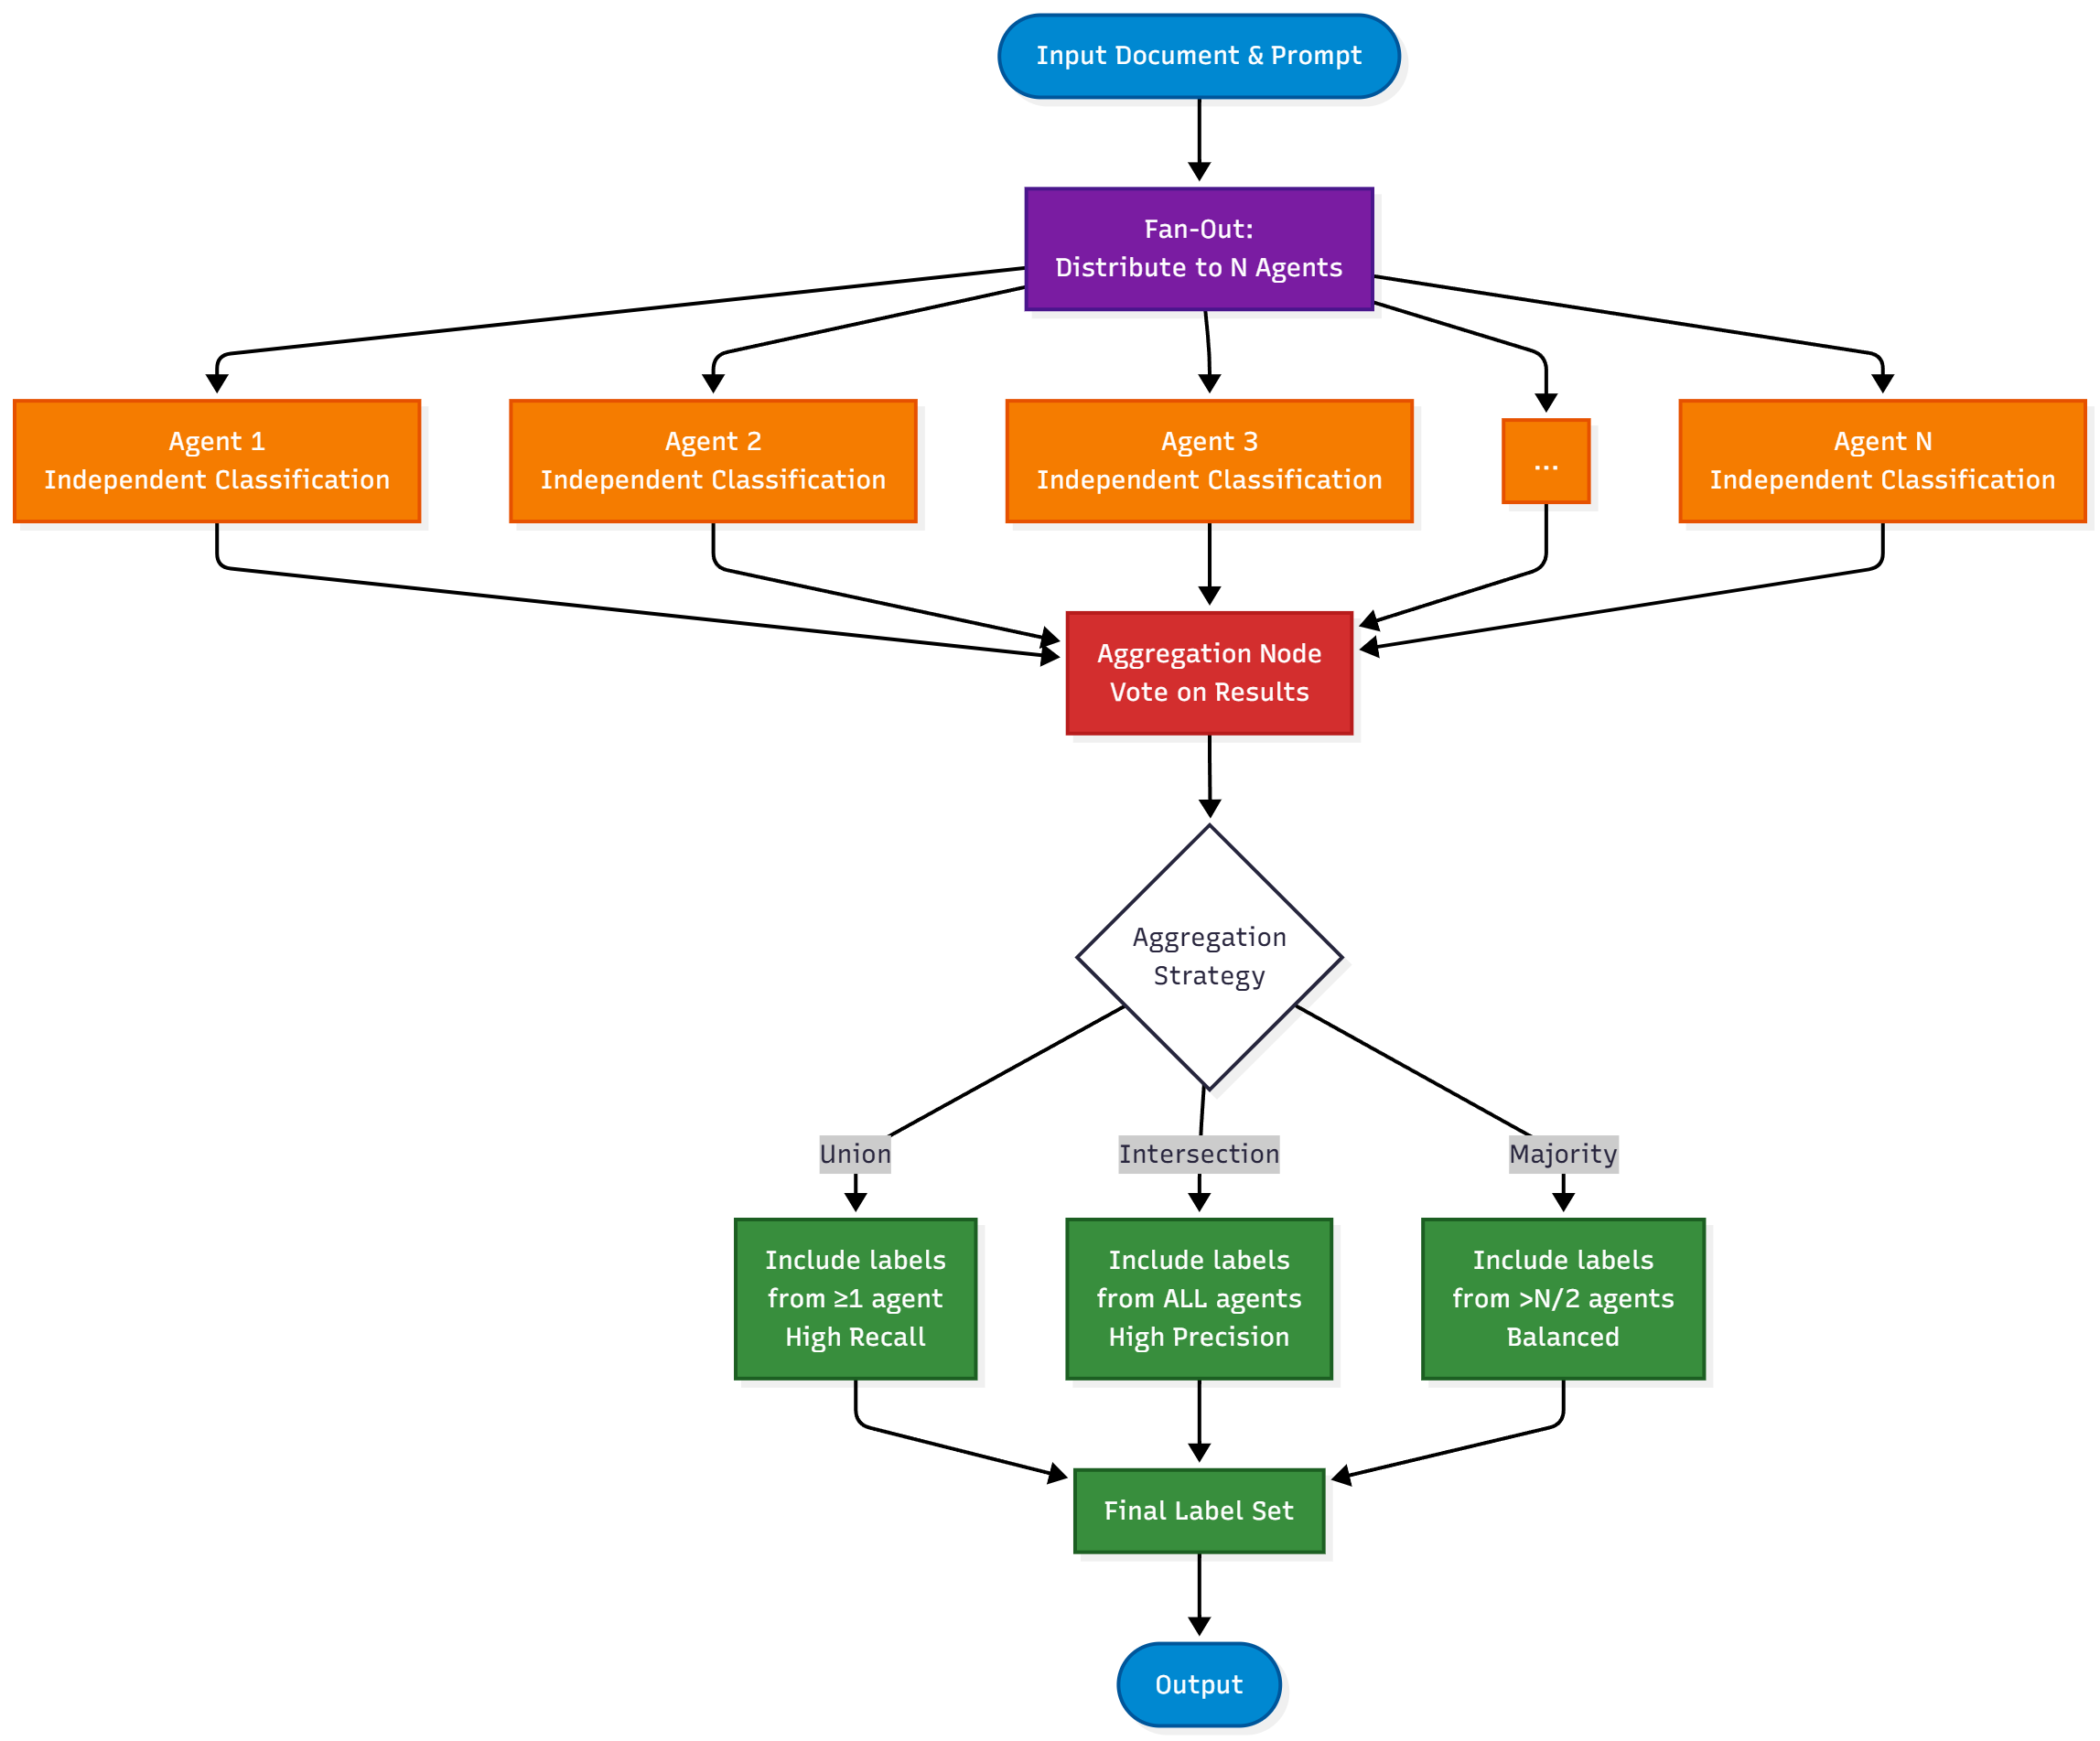
\includegraphics[height=12cm]{assets/diagrams/vote-based.png}
\caption{Agora multi-agent ensemble architecture. The framework distributes the classification task to $N$ independent agents in parallel (Fan-Out), aggregates their results using a voting mechanism (Fan-In), and produces a final label set based on the chosen aggregation strategy (Union, Intersection, or Majority Vote).}
\label{fig:vote_based_ensemble}
\end{figure*}

This ensemble approach directly addresses the single-point-of-failure issue observed in the Actor-Critic pipeline. Instead of relying on one critic's potentially noisy feedback, Agora relies on the statistical robustness of a majority decision, providing a more reliable and conceptually simpler method for improving classification quality.
